\chapter{Uncertainty Estimation and Calibration in Deep Neural Networks}

Deep Neural Networks (DNNs) have shown remarkable success in a wide range of fields. 
Although they have become increasingly appealing for high-risk domains such as medical image analysis 
or autonomous vehicle control, their deployment in \textbf{safety-critical} real-world applications 
remains limited.

This is because, in such contexts, we not only require the model to be accurate, but we also need to 
understand when the model is likely to be incorrect. For example, suppose we have a model that outputs 
the probability that a patient is affected by a brain tumor. Along with the prediction, the network 
also provides a value representing the reliability of that prediction. If this confidence value falls 
below a specified threshold, the prediction is discarded and a human expert is consulted instead.

The NNs are affected by several issues that lead to \textbf{uncertainty}. These problems are:
\begin{compactitemize}

    \item \textbf{Lack of Transparency}.  
    DNNs typically behave as \emph{black-box} models, meaning that their internal decision-making process is not easily interpretable by humans. This lack of transparency makes it difficult to understand why a model produces a certain output and prevents users from meaningfully assessing how confident the model is in its predictions.

    \item \textbf{Overconfident Predictions}.  
    Although neural networks output a distribution \(p(y \mid x, \theta)\) intended to represent class probabilities, they are often excessively confident even when their predictions are wrong. Model confidence is commonly inferred from the maximum softmax probability, but the softmax function is not a reliable measure of uncertainty: it can produce arbitrarily high values even for inputs that lie far outside the training distribution. Essentially, this problem occurs when the network assigns a score close to 1 to the predicted class; with such artificially high confidence, it becomes difficult to correctly estimate the true uncertainty.

    \item \textbf{Out-of-Distribution (OOD) Sensitivity}.  
    Due to their tendency toward overconfidence, DNNs often fail to distinguish between in-domain and out-of-domain samples. As a result, users or downstream systems may trust predictions that are actually meaningless or invalid. In high-risk contexts such as medical diagnosis or autonomous driving, this inability to detect OOD inputs can lead to dangerous failures without any warning signal.
    Due to this, we want that our model must recognize input that not belong to the original distribution.
    \item \textbf{Adversarial Vulnerability}.  
    Deep neural networks are sensitive to adversarial attacks—small, carefully crafted perturbations that are imperceptible to humans but cause the model to produce incorrect or unexpected outputs with high confidence. This vulnerability highlights fundamental weaknesses in the model’s robustness and further complicates the reliable estimation of uncertainty.
\end{compactitemize}
\begin{figure}[H]
    \centering
    \begin{minipage}{0.4\textwidth}
        \centering
        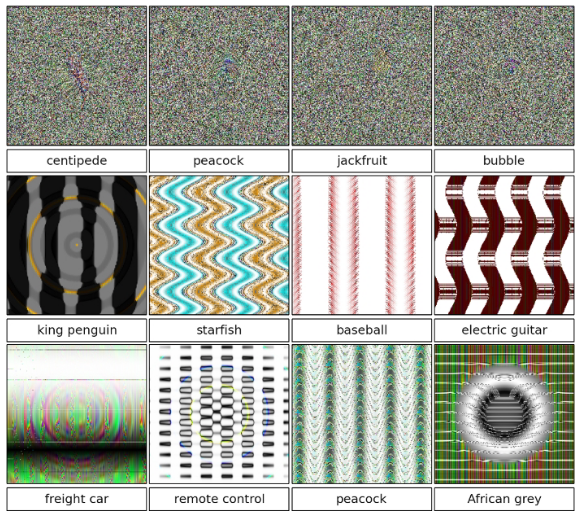
\includegraphics[width=\textwidth]{images/U2.png}
        \caption{OOD detection}
        \label{fig:Residuals}
    \end{minipage}
    \label{fig:TS_Residuals}
    \hfill
    \begin{minipage}{0.55\textwidth}
        \centering
        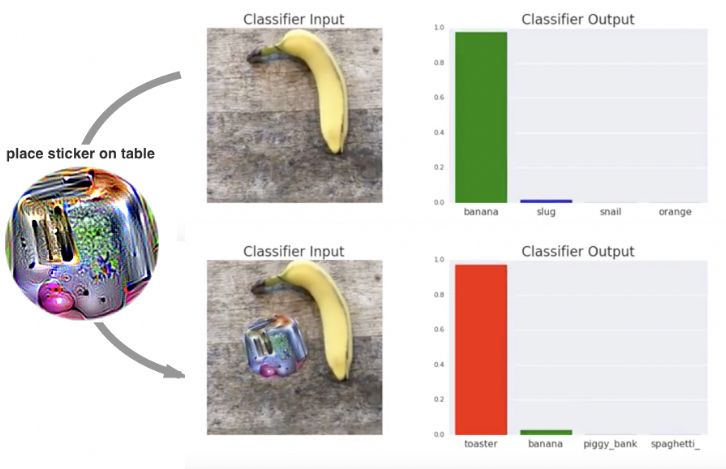
\includegraphics[width=\textwidth]{images/U3.png}
        \caption{Adversarial Attacks}
        \label{fig:Residuals}
    \end{minipage}
    \label{fig:TS_Residuals}
\end{figure}

To overcome these limitations and ensure safe decision-making in high-risk fields – including domains such as medical diagnosis, autonomous systems, and business intelligence – it is essential to provide \textbf{uncertainty estimates}, such that some predictions can be ignored or passed to human experts.

There are two different types of uncertainty. Let's see them:
\begin{compactitemize}

    \item \textbf{Aleatoric Uncertainty} (data uncertainty): arises from inherent noise, ambiguity, or class overlap in the data. It \textbf{persists regardless of how much data is collected}, as it is caused by randomness inherent in the data-generating process. This type of uncertainty \textbf{cannot be eliminated} even with more observations. It captures variability due to \textbf{measurement noise}, \textbf{ambiguous inputs}, or \textbf{naturally stochastic phenomena}. Aleatoric uncertainty occurs, for example, when the same input can correspond to multiple valid outputs, making the prediction task fundamentally ambiguous (e.g., label noise, sensor imprecision, or overlapping classes).  
    One example of this type of uncertainty is \textbf{stock price movement}: even if we were able to observe all relevant variables and theoretically make an accurate prediction, the data still contains inherent noise that makes the price evolution unpredictable.

    \item \textbf{Epistemic Uncertainty} (model uncertainty or systematic uncertainty): arises from a \textbf{lack of knowledge} about the underlying data distribution or model parameters. It is due to factors that one could, in principle, know but does not in practice. This uncertainty reflects the model’s \textbf{ignorance about the data}, often caused by limited, biased, or incomplete training sets. It captures uncertainty in the model’s parameters, structure, or ability to generalize to unseen data. Epistemic uncertainty also emerges when the model encounters unfamiliar situations that lie far from the training distribution. Unlike aleatoric uncertainty, \textbf{epistemic uncertainty can be reduced} by collecting more data or using better, more expressive models.

\end{compactitemize}

\section{Methods for Uncertainty Quantification}

\subsection{Deep Ensembles}
Deep Ensembles are one of the simplest and most effective approaches for uncertainty quantification in deep neural networks. The idea is to train multiple independent neural networks, each initialized with different random seeds and exposed to different shufflings of the training data. Because of this randomness, each model converges to a different local minimum, yet all solutions remain consistent with the data. The degree to which these models agree or disagree provides a natural estimate of \textbf{epistemic uncertainty}: if all models produce similar predictions, confidence is high; if they diverge, uncertainty increases.

\begin{wrapfigure}{r}{0.4\textwidth}
    \centering
    \vspace{-10pt}
    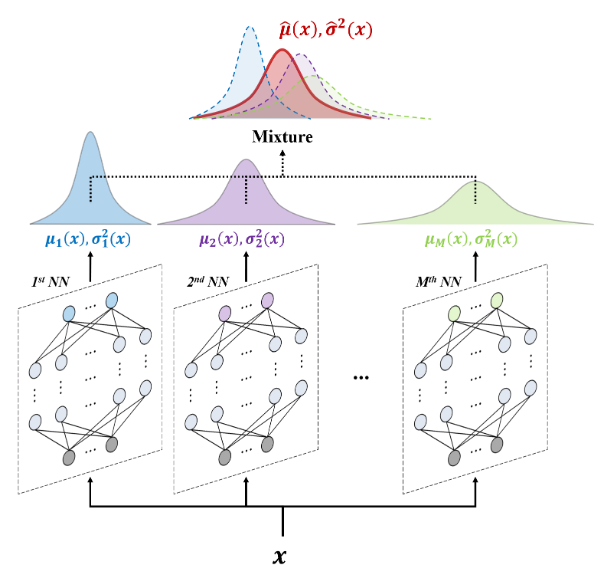
\includegraphics[width=\linewidth]{images/U4.png}
    \label{fig:Scaled Dot Product Attention}
    \vspace{-10pt}
\end{wrapfigure}
More precisely, when networks operate in regions of the input space that are well covered by training samples, they tend to produce similar outputs. However, in data-scarce regions, their predictions diverge, and this disagreement becomes a strong indicator of model uncertainty. Beyond simple ensembling, several tricks exist for improving uncertainty estimation, especially in regression tasks or robustness-oriented training paradigms.

\subsubsection{Predictive Uncertainty in Regression.}  
In standard regression settings, neural networks are typically trained to predict only the mean value $\mu(x)$ of the target variable, optimized through the Mean Squared Error (MSE) objective:
\[
\sum_{n=1}^{N} (y_n - \mu(x_n))^2.
\]
This formulation, however, does not capture any form of uncertainty, as it provides point estimates only. A more suitable approach is to predict both the mean $\mu(x)$ and the variance $\sigma^2(x) > 0$. Assuming a Gaussian likelihood
\[
y \sim \mathcal{N}(\mu(x), \sigma^2(x)),
\]
the model can be trained by minimizing the Negative Log-Likelihood (NLL):
\[
- \log p(y_n \mid x_n) = \log \sigma^2(x) + \frac{(y_n - \mu(x))^2}{\sigma^2(x)} + \text{const}.
\]
In practice, the variance is often constrained to be positive using a softplus activation or by adding a small constant (e.g., \(10^{-6}\)) for numerical stability.

\subsubsection{Merging Predictions in Ensembles (Classification).}  
Once the $M$ ensemble models have been trained, their predictions must be combined into a single predictive distribution. For classification, the ensemble is treated as a uniformly weighted mixture of models. The final predictive distribution is simply the average of the individual softmax probabilities:
\[
p_{E}(y \mid x) = \frac{1}{M} \sum_{m=1}^{M} p_{\theta_m}(y \mid x).
\]
To quantify model disagreement (epistemic uncertainty), one can compute the sum of Kullback–Leibler divergences between each model and the ensemble distribution:
\[
\sum_{m=1}^{M} \mathrm{KL}\big( p_{\theta_m}(y \mid x) \,\|\, p_{E}(y \mid x) \big).
\]

\subsubsection{Merging Predictions in Ensembles (Regression).}  
For regression tasks, each model in the ensemble outputs a predicted mean and variance, namely $\mu_m(x)$ and $\sigma_m^2(x)$ for $m = 1, \dots, M$. The ensemble prediction can be interpreted as a uniform mixture of $M$ Gaussian distributions. This mixture is often approximated by a single Gaussian with mean and variance given by:
\[
\mu_{\text{ens}}(x) = \frac{1}{M} \sum_{m=1}^{M} \mu_m(x),
\]
\[
\sigma_{\text{ens}}^{2}(x) 
= 
\frac{1}{M} \sum_{m=1}^{M} \left( \sigma_m^{2}(x) + \mu_m^{2}(x) \right) - \mu_{\text{ens}}^{2}(x)
=
\underbrace{
\frac{1}{M} \sum_{m=1}^{M} \sigma_m^{2}(x)
}_{\text{Aleatoric uncertainty}}
\;+\;
\underbrace{
\left[
\frac{1}{M} \sum_{m=1}^{M} \mu_m^{2}(x)
- \mu_{\text{ens}}^{2}(x)
\right]
}_{\text{Epistemic uncertainty}}.
\]
The resulting predictive variance includes both aleatoric and epistemic components, naturally decomposed through the ensemble formulation.

\subsubsection{Additional Technique: Adversarial Training.}  
Deep neural networks are known to be vulnerable to adversarial examples—small perturbations to the input that cause the model to produce incorrect but highly confident predictions. Adversarial training improves model robustness and often leads to smoother and more reliable predictive distributions.

The idea is to expose each ensemble model to adversarially perturbed inputs during training. A common approach is to generate adversarial samples using the Fast Gradient Sign Method (FGSM):
\[
x_{\text{adv}} = x + \epsilon \cdot \mathrm{sign}(\nabla_x L(x, y)),
\]
where $\epsilon$ controls the strength of the perturbation. The model is then trained on both clean and adversarial examples via the objective:
\[
\min_{\theta} \; \mathbb{E}_{(x, y)} \left[ L(f_{\theta}(x), y) \;+\; \lambda \cdot L(f_{\theta}(x_{\text{adv}}), y) \right],
\]
where $\lambda$ balances standard and adversarial training.  
When applied within an ensemble, adversarial training encourages each model to learn smoother decision boundaries, ultimately leading to more stable and calibrated uncertainty estimates.

\subsubsection{Limitations of Deep Ensembles}

Deep Ensembles are simple, empirically strong, and widely adopted for uncertainty quantification. 
However, despite their effectiveness, they also present several important limitations that motivate 
the search for more principled Bayesian approaches. The principal limitations are:
\begin{compactitemize}
    \item \textbf{High computational cost }: Deep Ensembles require training multiple independent neural networks from scratch, each with different random initializations and data shuffling. This leads to a computational overhead that grows linearly with the ensemble size. Memory usage also increases proportionally, making the method less suitable for large models or resource-constrained devices. Inference is slower as well, since it requires multiple forward passes—one for each ensemble member.

    \item \textbf{Limited diversity among ensemble members}: Although ensembles rely on model diversity to estimate epistemic uncertainty, in practice the members may converge to similar solutions, especially when trained on large datasets. As a consequence, the ensemble may underestimate epistemic uncertainty due to insufficient variability among the models.
\end{compactitemize}

Deep Ensembles show that averaging predictions of many diverse models improves uncertainty estimation. A natural question then arises: \emph{what if we could average not just a handful of models, but infinitely many?}  
One might consider generating an unbounded number of networks with random parameters and averaging their predictions. However, most randomly generated networks would produce meaningless outputs, yielding a poor approximation of meaningful uncertainty.

\subsubsection{Bayesian solution: weighted model averaging.}  
Instead of averaging arbitrary models, a Bayesian approach assigns higher probability to models whose parameters are more plausible given the dataset. Formally, the predictive distribution is defined as:
\[
p(y \mid x, D) = \int p(y \mid x, w) \, p(w \mid D) \, dw,
\]
where:
\begin{compactitemize}
    \item \(w\) are the model parameters,
    \item \(p(w \mid D)\) is the posterior distribution over parameters given the dataset \(D\),
    \item \(p(y \mid x, w)\) is the model likelihood,
    \item \(p(y \mid x, D)\) is the \emph{posterior predictive distribution} obtained by marginalizing over all plausible models.
\end{compactitemize}

Computing this integral exactly is intractable for modern neural networks. Therefore, Bayesian methods approximate it using \textbf{Monte Carlo} integration:
\[
p(y \mid x, D) \approx \frac{1}{J} \sum_{j=1}^{J} p(y \mid x, w_j), 
\qquad w_j \sim p(w \mid D).
\]

Two main families of methods are used to approximate samples from the posterior:
\begin{compactitemize}
    \item \textbf{Sampling-based methods}, such as Markov Chain Monte Carlo (MCMC).
    \item \textbf{Deterministic approximations}, such as Laplace approximations and Variational Inference.
\end{compactitemize}

\begin{infobox}[Connection to Deep Ensembles]
    Deep Ensembles can be interpreted as approximating the posterior \(p(w \mid D)\) with a set of 
    point masses located at different modes of the loss landscape. Although this is a crude approximation, 
    it is surprisingly effective in practice.
\end{infobox}

\subsubsection{Variational Inference (VI).}  
A popular deterministic Bayesian approach is Variational Inference. The idea is to approximate the true posterior \(p(w \mid D)\) with a simpler, tractable distribution \textbf{\(q_{\theta}(w)\)}, typically chosen within a parametric family (e.g., a Gaussian). The procedure is:
\begin{enumerate}
    \item Choose a family of approximate distributions \(q_{\theta}(w)\).
    \item Find the member \(q_{\theta}(w)\) that is closest to the true posterior by minimizing:
    \[
    \mathrm{KL}\big(q_{\theta}(w) \,\|\, p(w \mid D)\big).
    \]
    \item Once learned, samples \(w_j \sim q_{\theta}(w)\) can be drawn to approximate the predictive distribution:
    \[
    p(y \mid x, D) \approx \frac{1}{J} \sum_{j=1}^{J} p(y \mid x, w_j).
    \]
\end{enumerate}

Variational Inference can be seen as “turning integration into optimization,” making Bayesian model averaging computationally feasible while capturing epistemic uncertainty more rigorously than Deep Ensembles alone.

\subsection{Bayesian Neural Network (BNN)}
\begin{wrapfigure}{r}{0.6\textwidth}
    \centering
    \vspace{-10pt}
    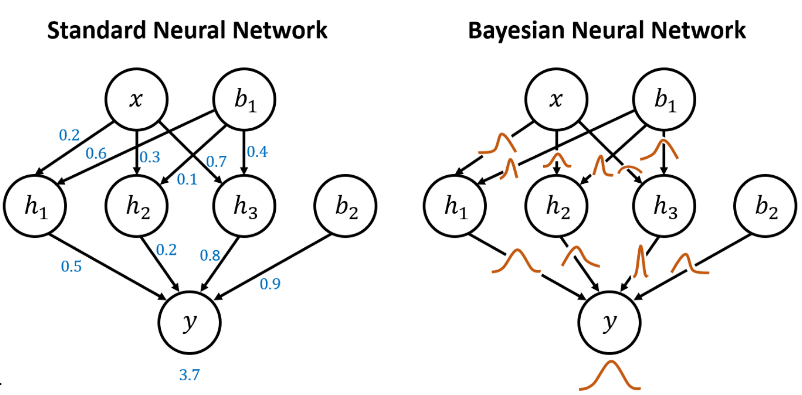
\includegraphics[width=\linewidth]{images/U5.png}
    \label{fig:Scaled Dot Product Attention}
    \vspace{-10pt}
\end{wrapfigure}

The approximate weight distribution $q_\theta(w) \approx p(w \mid D)$, introduced in the previous subsection, can be implemented through a \textbf{Bayesian Neural Network} (BNN). Unlike standard neural networks, which treat each parameter as a fixed value, BNNs represent every weight through a probability distribution. This leads to fundamental conceptual and practical differences between the two approaches.

\textbf{Standard Neural Networks}: In traditional neural networks, parameters are represented by single \emph{point estimates}. Training finds a specific set of weights $w^\ast$ that minimizes a given loss function. Because weights are fixed values, uncertainty is not explicitly modeled; the network produces deterministic outputs, and any regularization (e.g., weight decay, dropout) must be manually injected during training. As a consequence, these models cannot naturally quantify epistemic uncertainty and often rely on ensemble strategies to obtain more reliable predictions.

\textbf{Bayesian Neural Networks}: In BNNs, each weight is characterized by a probability distribution rather than a single value. Training starts by introducing a prior distribution $p(w)$ and updating it to a posterior $p(w \mid D)$ through Bayesian learning. This turns the model parameters into random variables and allows the BNN to explicitly capture \textbf{epistemic uncertainty}. Regularization arises naturally from the prior, reducing the need for manual techniques.  

Representing each weight through a distribution typically requires storing \emph{two} values—commonly a mean and a variance—doubling the memory footprint compared to standard networks. Despite this cost, BNNs offer an important advantage: because the model is \textbf{stochastic}, a single BNN can produce multiple plausible predictions by sampling different weight configurations from $q_\theta(w)$. This means that, unlike Deep Ensembles, we do not need to train many distinct deterministic networks; one stochastic model is sufficient to approximate Bayesian model averaging. Consequently, BNNs provide a theoretically grounded and memory-efficient alternative to ensembles for uncertainty estimation, particularly when combined with Variational Inference to approximate the intractable posterior distribution.

\begin{infobox}[Which are the most important weights?]
    The most important weights in the network are those with very small variance.
    This is intuitive: parameters with high variance do not significantly influence the output, since their value can fluctuate without affecting the prediction. 
    In contrast, parameters whose distribution is tightly concentrated around the mean are crucial for the model, as their value has a meaningful impact on the output.
\end{infobox}


\subsection{Bayes by BackPropagation}
\begin{wrapfigure}{r}{0.4\textwidth}
    \centering
    \vspace{-10pt}
    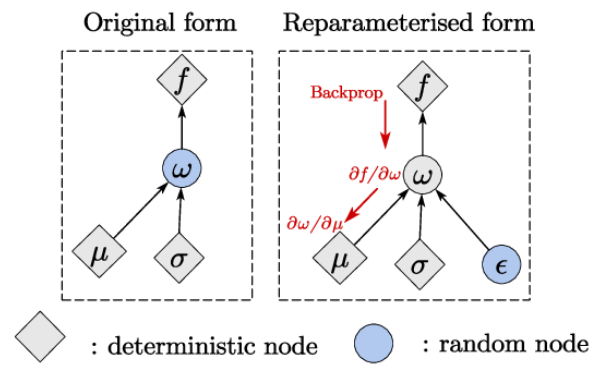
\includegraphics[width=\linewidth]{images/U6.png}
    \label{fig:Scaled Dot Product Attention}
    \vspace{-10pt}
\end{wrapfigure}
Bayes by Backprop  is one of the foundational methods for training Bayesian Neural Networks using variational inference combined with standard backpropagation. The key idea is to learn an approximate posterior distribution over the network weights instead of point estimates, enabling principled epistemic uncertainty estimation.

The method starts by introducing a prior distribution over the weights, typically chosen as an isotropic Gaussian:
\[
p(w) = \mathcal{N}(w \mid 0, \alpha^{-1} I),
\]
where $\alpha$ denotes the precision (i.e., the inverse variance).  
The variational posterior is modeled as another Gaussian distribution,
\[
q_\theta(w) = \mathcal{N}(w \mid \mu, \sigma^2),
\]
whose parameters $(\mu, \sigma)$ are learned during training. The training objective is to minimize the negative Evidence Lower Bound (ELBO):
\[
\mathcal{L}(\theta) = \mathrm{KL}(q_\theta(w) \,\|\, p(w)) - 
\mathbb{E}_{q_\theta(w)}[\log p(D \mid w)],
\]
which trades off model complexity (the KL term) and data fit (the likelihood term).

To make the optimization tractable, Bayes by Backprop uses the \textbf{reparameterization trick}. Instead of sampling $w$ directly from $q_\theta(w)$, the weight is expressed as:
\[
w = \mu + \sigma \odot \epsilon, \qquad \epsilon \sim \mathcal{N}(0, I).
\]
This allows gradients to propagate through $\mu$ and $\sigma$ (or through a transformed parameter $\rho$ such that $\sigma = \log(1 + e^\rho)$), enabling end-to-end training using standard backpropagation.

During training, weights are resampled at each forward pass, turning the model into a stochastic network. The likelihood term is estimated by sampling multiple weight realizations from $q_\theta(w)$ and computing, for each of them, the log-likelihood (e.g., cross-entropy for classification). For a minibatch $B$, the loss becomes:
\[
\mathcal{L}_B = 
\sum_{(x,y) \in B}
\mathbb{E}_{q_\theta(w)}[-\log p(y \mid x, w)]
\;+\;
\mathrm{KL}(q_\theta(w) \,\|\, p(w)).
\]

This formulation enables a single Bayesian neural network to approximate Bayesian model averaging, eliminating the need for training multiple deterministic networks as required by Deep Ensembles.


\subsubsection{Two Practical Tricks for BNN Training}

Training Bayesian neural networks via variational inference can be challenging in practice. Two widely used techniques help stabilize optimization and improve the quality of the posterior approximation.

\textbf{1. KL Re-weighting for minibatch training.}  
Instead of applying the KL divergence term uniformly during training, its contribution is scaled by a minibatch-dependent factor $\pi_i$. A common strategy is to let $\pi_i$ decay from $1$ to $0$ as training progresses:
\[
\mathcal{L}^{(i)} = \pi_i \, \mathrm{KL}(q_\theta(w) \,\|\, p(w)) 
\;-\; 
\mathbb{E}_{q_\theta(w)}[\log p(D \mid w)].
\]
Early in training, the posterior is strongly influenced by the prior, which prevents unstable updates when the model has seen very little data. As more minibatches are processed, the likelihood term becomes dominant, allowing the data to take over and refine the approximate posterior. This annealing strategy often leads to better convergence and more stable updates of the variance parameters.

\textbf{2. Mixture Priors.}  
Instead of using a single Gaussian prior, a more flexible choice is a mixture of two Gaussians:
\[
p(w_j) = 
\pi \, \mathcal{N}(w_j \mid 0, \sigma_1^2)
\;+\;
(1 - \pi) \, \mathcal{N}(w_j \mid 0, \sigma_2^2),
\]
where the first component has a large variance ($\sigma_1 \gg 1$), providing heavy tails, and the second component has a very small variance ($\sigma_2 \ll 1$), encouraging many weights to concentrate tightly around zero.  
This prior promotes sparsity and gives the posterior more flexibility, allowing the BNN to model both highly relevant weights (captured by the broad Gaussian) and irrelevant ones (captured by the narrow Gaussian). Mixture priors often lead to better posterior approximations and improved uncertainty estimates, especially in overparameterized networks.

\subsection{Dropout}
\begin{wrapfigure}{r}{0.35\textwidth}
    \centering
    \vspace{-10pt}
    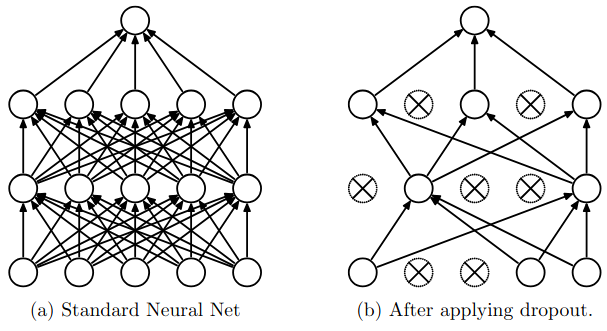
\includegraphics[width=\linewidth]{images/U7.png}
    \label{fig:Scaled Dot Product Attention}
    \vspace{-10pt}
\end{wrapfigure}
Dropout is a regularization technique originally introduced to reduce overfitting and prevent co-adaptation of neurons in standard neural networks. During training, each hidden unit is independently \textit{dropped} (i.e., set to zero) with probability $p$. For each mini-batch, a binary mask $m^{(l)}$ is sampled for every layer $l$:
\[
h_{\text{dropped}}^{(l)} = m^{(l)} \odot h^{(l)},
\qquad
m^{(l)}_i \sim \text{Bernoulli}(1 - p).
\]
This forces the network to learn redundant and robust feature representations, since the model cannot rely on the presence of any single neuron.

At inference time, the dropout noise is typically \emph{disabled}, meaning that the full network is used without masking any activations. To ensure consistency with the expected activations during training, outputs are rescaled by a factor of $(1 - p)$, which maintains the same magnitude as in the stochastic training regime.

Thus, dropout acts as an implicit ensemble of many subnetworks, improving robustness and reducing overfitting at essentially no additional computational cost during training.


\subsection{Monte Carlo Dropout (MC Dropout)}
\begin{wrapfigure}{r}{0.4\textwidth}
    \centering
    \vspace{-10pt}
    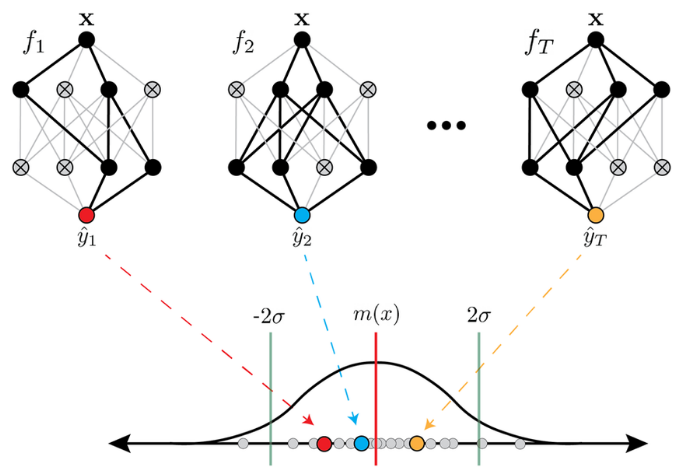
\includegraphics[width=\linewidth]{images/U8.png}
    \label{fig:Scaled Dot Product Attention}
    \vspace{-10pt}
\end{wrapfigure}

BNNs are very useful, but they have a drawback: they require changing the training paradigm and training an entirely different type of network. In many practical scenarios, however, we already have a standard deterministic neural network, and it would be convenient to have a method to make such a network stochastic without redesigning it. This can be achieved through MC Dropout.
Monte Carlo Dropout \ extends the classical dropout mechanism to provide an efficient approximation to Bayesian inference in neural networks. The key idea is to interpret dropout as a variational approximation to a Bayesian neural network, enabling uncertainty estimation without the heavy computational cost of full Bayesian methods.

\textbf{Idea.}  
Instead of disabling dropout at test time, MC Dropout keeps it active and performs multiple stochastic forward passes. Each pass corresponds to sampling a different dropout mask, effectively drawing a sample from an approximate posterior over the model weights.

\textbf{Procedure.}
\begin{enumerate}
    \item Train a standard neural network using dropout as usual.
    \item At test time, leave dropout \emph{enabled} instead of turning it off.
    \item Perform $T$ stochastic forward passes, each with newly sampled dropout masks:
    \[
    f^{(t)}(x) = f(x; \theta, m_1^{(t)}, \ldots, m_L^{(t)}),
    \qquad t = 1, \ldots, T.
    \]
    \item Estimate the predictive mean:
    \[
    \hat{\mu}(x) = \frac{1}{T} \sum_{t=1}^{T} f^{(t)}(x).
    \]
    \item Estimate the predictive covariance:
    \[
    \widehat{\mathrm{Cov}}[y \mid x, D] = 
    \frac{1}{T} \sum_{t=1}^{T} 
    f^{(t)}(x)f^{(t)}(x)^\top
    - 
    \hat{\mu}(x)\hat{\mu}(x)^\top 
    + \tau^{-1} I,
    \]
    where $\tau^{-1}$ is the assumed observation noise variance.
\end{enumerate}

The variability across the stochastic outputs $f^{(t)}(x)$ captures \textbf{epistemic uncertainty}, since it reflects sensitivity to different sampled subnetworks. Model uncertainty can be quantified through the entropy of the predictive distribution, variation ratios, or the predictive covariance above.

The \textbf{Benefits} of the Mont-Carlo Dropout are:
\begin{compactitemize}
    \item No modification to the training procedure is required.
    \item Computational overhead is modest: only multiple forward passes are needed.
    \item Provides a practical approximation to Bayesian uncertainty without training multiple deterministic models (as in Deep Ensembles).
\end{compactitemize}

\section{Reliable Uncertainty Measures}

\subsection{Confidence from the Predicted Probability}

A very common and simple approach to estimate how confident a neural network is about a prediction is to look at the highest output of the Softmax layer.
Given a classification problem with $K$ classes, the network produces a vector of predicted probabilities
\[
\mathbf{p}(x) = [p_1(x), p_2(x), \dots, p_K(x)],
\]
where $p_k(x)$ represents the predicted probability that the input $x$ belongs to class $k$.

For instance, consider the prediction
\[
[0.05,\, 0.10,\, 0.80,\, 0.05].
\]
The highest value is $0.80$, corresponding to class 3. In this case, we would say that the model is \emph{80\% confident} that the input belongs to class 3.

This notion of confidence is intuitive. If the maximum predicted probability is close to $1$, the model appears very certain about its decision. Conversely, if the maximum probability is low, for example around $0.4$ or $0.5$, the prediction is ambiguous and several classes compete with similar scores.

However, this interpretation relies on the implicit assumption that Softmax outputs represent meaningful probabilities. Unfortunately, this assumption is often violated.

\subsection{Miscalibration}
\begin{wrapfigure}{r}{0.5\textwidth}
    \centering
    \vspace{-10pt}
    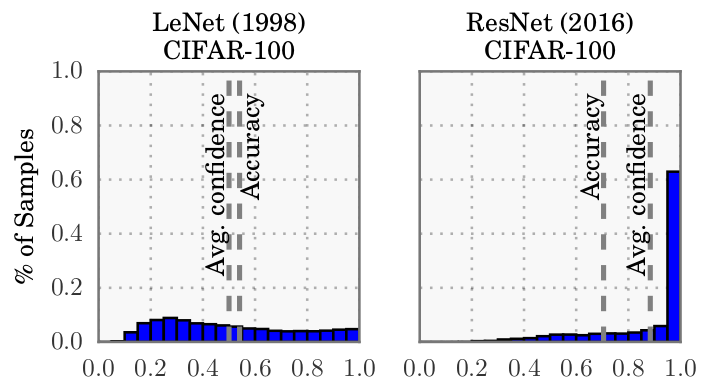
\includegraphics[width=\linewidth]{images/V1.png}
    \label{fig:Scaled Dot Product Attention}
    \vspace{-10pt}
\end{wrapfigure}
The main limitation of using the maximum Softmax probability as a confidence estimate is that this quantity does not necessarily reflect the true probability of making a correct prediction.

Given a dataset $\{x_i\}_{i=1}^N$, the confidence of a model on a single input $x_i$ is typically defined as
\[
\mathrm{conf}(x_i) = \max_{k \in \{1,\dots,K\}} p_\theta(y = k \mid x_i),
\]
that is, the maximum predicted probability among all classes.

At the dataset level, model confidence is often summarized by the \emph{average confidence}, defined as
\[
\frac{1}{N} \sum_{i=1}^{N} \max_{k \in \{1,\dots,K\}} p_\theta(y = k \mid x_i).
\]

If the model were perfectly calibrated, this average confidence would closely match the empirical accuracy. In practice, however, modern neural networks frequently violate this property. The model may assign very high confidence scores to its predictions even when a significant fraction of them are incorrect.

This discrepancy shows that Softmax outputs should not be interpreted as true posterior probabilities. Instead, they represent normalized scores whose scale is influenced by architectural choices and training procedures. As a result, relying solely on the maximum predicted probability can lead to misleading uncertainty estimates, especially in deep and overparameterized models.

This behavior is largely a consequence of how neural networks are trained.
In supervised classification, the ground-truth label is typically encoded as a one-hot vector, for example
\[
[0,\,0,\,1,\,0,\,0],
\]
where the correct class is assigned probability $1$ and all the others probability $0$.

During training, the network is optimized to match this target distribution, usually by minimizing the cross-entropy loss. As a result, the model is explicitly encouraged to concentrate as much probability mass as possible on a single class, pushing the maximum predicted probability toward $1$.

However, this one-hot target does not represent the true underlying uncertainty of the data-generating process. In many cases, the real posterior distribution over classes is much softer, but the network is never exposed to this information. Consequently, the model learns to approximate an artificially sharp distribution, which explains why high confidence values are often produced even when the prediction is incorrect.

This mismatch between the learned confidence scores and the true likelihood of correctness directly leads to miscalibration.

This effect is further amplified by model complexity.
Smaller and simpler networks tend to produce smoother and more conservative confidence estimates, which are often more reliable. Their confidence values are less extreme and closer to the empirical accuracy, making them, in practice, more \emph{honest} about their uncertainty.

In contrast, large and highly overparameterized architectures, such as very deep models, have sufficient capacity not only to fit the training data correctly but also to push the predicted probabilities toward extreme values. In this regime, the network learns to strongly commit to its predictions, assigning high confidence scores even in situations where uncertainty should be present.

This behavior can be interpreted as a form of overfitting at the level of confidence rather than accuracy. While the overall classification performance may improve, the predicted probability distribution becomes increasingly sharp and less representative of the true underlying uncertainty. As a consequence, the model appears highly confident even when it is wrong.

For this reason, older or smaller architectures often exhibit better calibration: not because they are more accurate, but because their limited capacity prevents them from producing overly confident predictions. Their confidence estimates are smoother, more moderate, and therefore more aligned with the true likelihood of correctness.

\subsubsection{A Calibration Question}

Consider the following question. Suppose we collect all the samples in a dataset for which the model’s confidence, defined as the maximum predicted probability, lies in the interval $[0.45, 0.55]$, that is, close to $0.5$.

If we take 100 such samples, how many of them should we expect to be classified correctly?

The answer is \emph{approximately 50}, but this holds if and only if the model is perfectly calibrated. In a well-calibrated model, predictions with confidence $c$ are correct approximately $c \times 100\%$ of the time. When this property does not hold, the confidence values cannot be trusted as measures of uncertainty.

\subsection{Reliability Diagrams}

Reliability diagrams are a standard tool used to visualize and evaluate the calibration of a model. The idea is to group predictions into confidence bins, for example $[0.0,0.1], [0.1,0.2], \dots, [0.9,1.0]$, according to their maximum predicted probability.

For each bin, two quantities are computed: the average confidence of the samples in the bin and the empirical accuracy, defined as the fraction of correctly predicted samples. These values are then plotted against each other.

If a model is perfectly calibrated, the points in the reliability diagram lie on the diagonal line $y=x$. Any deviation from this diagonal indicates miscalibration. When the accuracy is consistently below the confidence, the model is overconfident; when it is above, the model is underconfident.
\begin{figure}[H]
    \centering
    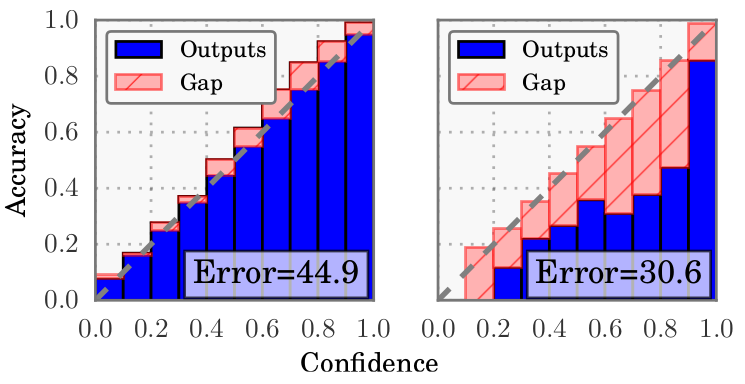
\includegraphics[width=0.5\textwidth]{images/V2.png}
    \label{fig:Scaled Dot Product Attention}
\end{figure}

Empirical results on datasets such as CIFAR-100 show that deep architectures like ResNet (right in the image above), despite achieving significantly higher accuracy than older models such as LeNet (left in the image above), are often much more miscalibrated. In contrast, simpler and older networks tend to produce confidence estimates that better reflect their true correctness likelihood, even if their overall accuracy is lower.

\subsection{Expected Calibration Error (ECE)}

While reliability diagrams provide an intuitive and visual way to assess calibration, it is often useful to summarize miscalibration with a single numerical metric. The most commonly used measure for this purpose is the \emph{Expected Calibration Error} (ECE).

The goal of ECE is to quantify how far the model’s predicted confidence is from its actual empirical accuracy. To compute ECE, predictions are first partitioned into $M$ confidence bins, typically obtained by dividing the interval $[0,1]$ into equally spaced ranges such as $[0.0,0.1], [0.1,0.2], \dots, [0.9,1.0]$. Each sample is assigned to a bin based on its predicted confidence, defined as the maximum Softmax probability.

For each bin $B_m$, two quantities are computed. The accuracy of the bin is defined as
\[
\mathrm{acc}(B_m) = \frac{1}{|B_m|} \sum_{x_i \in B_m} \mathbb{I}\{\hat{y}_i = y_i\},
\]
that is, the fraction of correctly classified samples in the bin. The average confidence of the bin is defined as
\[
\mathrm{conf}(B_m) = \frac{1}{|B_m|} \sum_{x_i \in B_m} \max_k p_\theta(y = k \mid x_i).
\]

The Expected Calibration Error is then defined as a weighted average of the absolute difference between accuracy and confidence across all bins:
\[
\mathrm{ECE} = \sum_{m=1}^{M} \frac{|B_m|}{n} \, \big| \mathrm{acc}(B_m) - \mathrm{conf}(B_m) \big|,
\]
where $n$ is the total number of samples.

An ECE value equal to zero corresponds to perfect calibration, meaning that for every confidence level the predicted confidence matches the empirical accuracy. Larger ECE values indicate increasing degrees of miscalibration. Intuitively, ECE measures the average vertical distance between the reliability diagram and the diagonal line representing ideal calibration.
\begin{figure}[H]
    \centering
    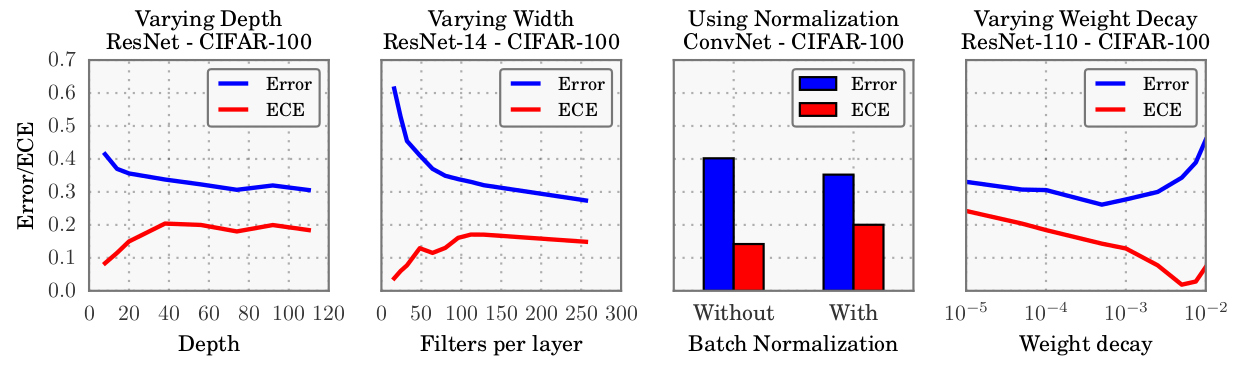
\includegraphics[width=1\textwidth]{images/U9.png}
    \label{fig:MHA2}
\end{figure}

\subsection{Temperature Scaling}

Temperature scaling is a simple yet effective post-processing technique used to improve the calibration of a trained classifier without affecting its predictive accuracy. The key idea is to modify the confidence of the predictions while leaving the predicted class unchanged.

Let $\mathbf{z} = (z_1, \dots, z_K)$ denote the logits produced by the network before the Softmax layer. Temperature scaling introduces a single scalar parameter $T > 0$, called the \emph{temperature}, and rescales the logits before applying Softmax:
\[
p_\theta(y = k \mid x) =
\frac{\exp(z_k / T)}{\sum_{j=1}^{K} \exp(z_j / T)}.
\]
\begin{wrapfigure}{r}{0.4\textwidth}
    \centering
    \vspace{-10pt}
    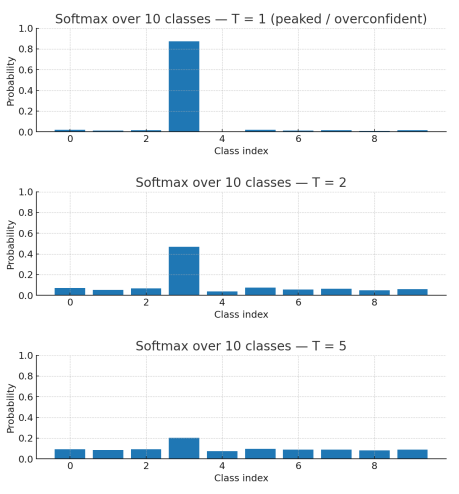
\includegraphics[width=\linewidth]{images/U10.png}
    \label{fig:Scaled Dot Product Attention}
    \vspace{-10pt}
\end{wrapfigure}
When $T = 1$, the standard Softmax is recovered. For $T > 1$, the logits are divided by a value greater than one, resulting in a softer probability distribution. In this case, the maximum predicted probability is reduced, leading to lower and more conservative confidence scores. Importantly, the ordering of the logits is preserved, so the predicted class does not change.

The temperature parameter is learned after training, using a held-out validation set. Specifically, $T$ is optimized by minimizing the negative log-likelihood of the validation data, while keeping all model parameters fixed. As a consequence, temperature scaling does not modify the classifier itself but only rescales the confidence values of its predictions.

An important advantage of temperature scaling is that it improves calibration without altering the model’s accuracy. Since the predicted labels remain identical, performance metrics such as accuracy are unchanged, while the predicted probabilities become more aligned with the empirical correctness likelihood.


\subsection{Brier Score}

The Brier Score is a commonly used metric to evaluate the quality of probabilistic predictions in both binary and multi-class classification settings. Unlike accuracy, which only evaluates whether the predicted class is correct, the Brier Score explicitly measures how close the predicted probability distribution is to the true target distribution.

Formally, for a dataset of $N$ examples and $K$ classes, the Brier Score is defined as
\[
\mathrm{BS} = \frac{1}{N} \sum_{i=1}^{N} \sum_{k=1}^{K}
\big( p_{i,k} - y_{i,k} \big)^2,
\]
where $p_{i,k}$ denotes the probability predicted by the model for class $k$ on example $i$, and $y_{i,k}$ is the corresponding one-hot encoded ground-truth label.

The Brier Score computes the mean squared difference between predicted probabilities and the true outcomes. Intuitively, it penalizes both incorrect predictions and poorly calibrated confidence estimates. Confident but wrong predictions result in a large penalty, while well-calibrated and accurate probability estimates yield low scores.

Lower Brier Score values indicate better probabilistic predictions. In the binary classification setting, the score ranges from $0$, corresponding to perfect predictions, to $1$, corresponding to maximally incorrect and overconfident predictions. In the multi-class case, the range depends on the number of classes but the interpretation remains the same.

An important property of the Brier Score is that it is a \emph{proper scoring rule}. This means that the score is minimized when the predicted probabilities match the true underlying data distribution, thereby encouraging honest and well-calibrated probability estimates. Moreover, the Brier Score is sensitive not only to calibration but also to refinement, capturing both how accurate and how sharp the predicted probability distributions are.

\subsection{Out-of-Distribution Detection}

Out-of-distribution (OOD) detection aims at identifying inputs that differ significantly from the data distribution used during training. The objective is to detect these inputs at test time so that the model can abstain from making a prediction or trigger a fallback mechanism.

This problem is particularly important because deep neural networks are known to produce highly confident predictions even for inputs that are completely unrelated to the training data, such as random noise or samples coming from a different domain. In safety-critical applications, including medical diagnosis and autonomous driving, such overconfident behavior on OOD inputs can lead to severe and potentially dangerous errors.

OOD detection therefore complements uncertainty estimation and calibration: even a well-calibrated model on in-distribution data may behave unpredictably when evaluated far outside its training support.

\subsubsection{ODIN}

ODIN is a post-hoc method for OOD detection that operates on a trained classifier, without requiring retraining or architectural changes. Its goal is to increase the separation between in-distribution (ID) and out-of-distribution samples by exploiting differences in how the model reacts to small input perturbations.

The method combines two key components. First, temperature scaling is applied to the logits, using a temperature value $T > 1$ to soften the Softmax output. This reduces overconfidence and amplifies relative differences in confidence between ID and OOD inputs.

Second, a small, carefully chosen perturbation is added to the input. Specifically, the input $x$ is modified as
\[
\tilde{x} = x + \epsilon \, \mathrm{sign} \left( \nabla_x \log p(y_{\max} \mid x; T) \right),
\]
where $y_{\max}$ is the class with maximum predicted probability under temperature-scaled Softmax, and $\epsilon$ controls the perturbation magnitude.

This step resembles an adversarial update, but with the opposite objective: instead of reducing confidence, the perturbation is designed to increase the model’s confidence in its current prediction.

The key intuition behind ODIN is that this perturbation has a different effect on ID and OOD samples. For in-distribution inputs, the perturbation tends to align with meaningful features learned during training, producing a noticeable increase in the maximum Softmax probability. In contrast, OOD inputs typically lie in regions of the input space that the model does not understand well. As a consequence, even after the perturbation, their logits do not align strongly with any learned pattern, and the Softmax confidence increases only marginally.

At test time, both temperature scaling and input perturbation are applied, and the maximum Softmax probability computed on $\tilde{x}$ is used as an OOD score. By comparing this score to a predefined threshold, the model can flag inputs that are likely to be out-of-distribution. The combined effect of temperature scaling and input perturbation widens the confidence gap between ID and OOD samples, making them easier to separate.
